\documentclass[journal]{IEEEtran}

\ifCLASSINFOpdf
  \usepackage[pdftex]{graphicx}
\else
  \usepackage[dvips]{graphicx}
\fi

\ifCLASSOPTIONcompsoc
  \usepackage[caption=false,font=normalsize,labelfont=sf,textfont=sf]{subfig}
\else
  \usepackage[caption=false,font=footnotesize]{subfig}
\fi

\usepackage{amsmath,amsfonts,amsthm,amssymb}

\usepackage{url}
\usepackage{multirow}



\hyphenation{StarCraft com-pe-ti-ti-ve par-ti-ci-pants}

\begin{document}

\title{The Current State of \\StarCraft AI Competitions and Bots}

\author{Michal~\v{C}ertick\'{y} and~David~Churchill% <-this % stops a space
\thanks{Michal \v{C}ertick\'{y} is with the Artificial Intelligence Center at Faculty of Electrical Engineering, Czech Technical University in Prague. Email:~\tt{certicky@agents.fel.cvut.cz}}% <-this % stops a space
\thanks{David Churchill is with Department of Computer Science, Memorial University of Newfoundland. Email:~\tt{dave.churchill@gmail.com}}% <-this % stops a space
}

% The paper headers
%\markboth{Journal of \LaTeX\ Class Files,~Vol.~14, No.~8, August~2015}%
%{Shell \MakeLowercase{\textit{et al.}}: Bare Demo of IEEEtran.cls for IEEE Journals}
% The only time the second header will appear is for the odd numbered pages
% after the title page when using the twoside option.
% 
% *** Note that you probably will NOT want to include the author's ***
% *** name in the headers of peer review papers.                   ***
% You can use \ifCLASSOPTIONpeerreview for conditional compilation here if
% you desire.


% make the title area
\maketitle
\begin{abstract}
Real-Time Strategy (RTS) games have become an increasingly popular test-bed for modern artificial intelligence techniques. With this rise in popularity has come the creation of several annual competitions, in which AI agents (bots) play the full game of StarCraft: Broodwar by Blizzard Entertainment. The three major annual StarCraft AI Competitions are the Student StarCraft AI Tournament (SSCAIT), the Computational Intelligence in Games (CIG) competition, and the Artificial Intelligence and Interactive Digital Entertainment (AIIDE) competition. In this paper we will give an overview of the current state of these competitions, and the bots that compete in them. 
\end{abstract}

% For peer review papers, you can put extra information on the cover
% page as needed:
% \ifCLASSOPTIONpeerreview
% \begin{center} \bfseries EDICS Category: 3-BBND \end{center}
% \fi
%
% For peerreview papers, this IEEEtran command inserts a page break and
% creates the second title. It will be ignored for other modes.
\IEEEpeerreviewmaketitle


\section{Introduction}\label{secIntro}

Real-time Strategy (RTS) games are a genre of video games in which players manage economic and strategic tasks by gathering resources, building bases, increase their military power by researching new technologies and training units, and lead them into battle against their opponent(s). They serve as an interesting domain for Artificial Intelligence (AI) research and education, since they represent a well-defined, complex adversarial systems \cite{Buro2004} which pose a number of interesting AI challenges in the areas of planning, dealing with uncertainty, domain knowledge exploitation, task decomposition, spatial reasoning, and machine learning \cite{Survey2013}.

Unlike turn-based abstract board games like chess and go, which can already be played by AI at super-human skill levels, RTS games are played in \textit{real-time}, meaning the state of the game will continue to progress even if the player takes no action, and so actions must be decided in fractions of a second. In addition to that, individual turns in RTS games (game frames) can consist of issuing simultaneous actions to hundreds of units at any given time \cite{buro2012real}. This, together with their partially observable and non-deterministic nature, makes RTS game genre one of the hardest game AI challenges today, attracting the attention of the academic research community, as well as commercial companies. For example, Facebook AI Research, Microsoft, and Google DeepMind have all recently expressed interest in using the most popular RTS game of all time: Starcraft as a test environment for their AI research \cite{gibney2016google}. 

Meanwhile, the academic community has been using StarCraft as a domain for AI research since the advent of the Brood War Application Programming Interface (BWAPI) in 2009 \cite{heinermann2013bwapi}. BWAPI allows programs to interact with the game engine directly to play autonomously against human players or against other programs (bots). The introduction of BWAPI gave rise to numerous scientific publications over last 8 years, dealing with all kinds of sub-problems inherent to RTS games. A comprehensive overview can be found in \cite{churchill2016starcraft}, \cite{ontanon2015rts} or \cite{Survey2013}.

In addition to AI research, StarCraft and BWAPI are often used for educational purposes as part of AI-related  courses at universities, including UC Berkeley (US), Washington State University (US), University of Alberta (CA), Comenius University (SK), Czech Technical University (CZ), University of \v{Z}ilina (SK) and most recently Technical University Delft (NL), where a new course entitled ``Multi-agent systems in StarCraft'' has been opened for over 200 students. The educational potential of StarCraft has recently been extended even further, when Blizzard Entertainment released the game entirely for free in April 2017.

Widespread use of StarCraft in research and education has lead to a creation of three annual StarCraft AI competitions existing until today. The first competition was organized at the University of California, Santa Cruz in 2010 as part of the AAAI Artificial Intelligence and Interactive Digital Entertainment (AIIDE) conference program. The following year gave rise to other two annual competitions -- Student StarCraft AI Tournament (SSCAIT), organized as a standalone long-term event at Comenius University in Bratislava and Czech Technical University in Prague, and CIG StarCraft AI competition collocated with IEEE Computational Intelligence in Games (CIG) conference.

%- in this paper, we will talk about those competions and provide latest news 
%- and then, we will also talk about the state of the research - we'll bots describe current bots and AI methods they use
In this paper, we will talk about these three major StarCraft AI competitions and provide the latest updates on each of them, with the following 3 sections detailing the SSCAIT, AIIDE, and CIG Starcraft AI Competitions. We will also take a closer look at the state of the research and briefly describe current participants (bots) and AI methods they use. Finally, we will introduce the open-source Tournament Manager Software powering the competitions. 




%%%%%%%%%%%%%%%%%%%%%%%%%%%%%%%%%%%%%%%%%%%%%%%%%%%%%%%%%%%%%%%%%%%%%%%%%%%%%
\section{SSCAIT: Student StarCraft\\ AI Tournament}\label{subsecSSCAIT}

The Student StarCraft AI Tournament (SSCAIT) is the StarCraft AI competition with the highest number of total participants. There are three fundamental differences between SSCAIT and the remaining two competitions:
\begin{enumerate}
  \item SSCAIT is an online-only event. Unlike AIIDE or CIG, it is not co-located with a scientific conference / event. \item There are two phases of SSCAIT each year: a~competitive {\em tournament phase}, lasting for up to four weeks and a {\em ladder phase} which runs for the rest each year. In other words, SSCAIT is live at all times with only a few short interruptions for maintenance.
  \item Games are played one at a time and are publicly streamed live on Twitch.tv.\footnote{http://www.twitch.tv/sscait} and SmashCast.tv. The AIIDE and CIG competitions instead play as many games as possible at maximum speed, with no broadcast.
\end{enumerate}

SSCAIT's {\em tournament phase} takes place every winter in late December and early January. 
%At the time of writing of this paper, SSCAIT 2017/18 tournament was in progress with 78 participants. Since the 2017/18 results are still incomplete, we cover the results of previous SSCAIT year.

\begin{figure}[t]
  \centering
  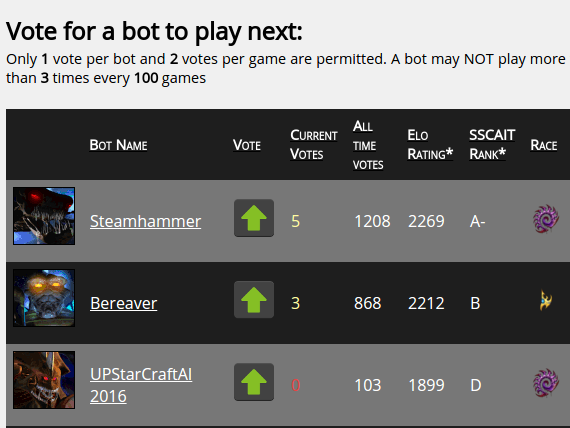
\includegraphics[width=1\columnwidth]{fig/sscait-voting.png}
  \caption{A web-based interface allowing SSCAIT viewers and bot programmers to vote for the next ladder match.}
  \label{figSSCAITvoting}
\end{figure}

%%%%%%%%%%%%%%%%%%%%%%%%%%%%%%%%%%%%%%%%%%%%%%%%%%%%%%%%%%%%%%%%%%%%%%%%%%%%%
\subsection{SSCAIT History}

The first SSCAIT was organized in 2011 by Michal \v{C}ertick\'{y}, as a part of the ``Fundamentals of Artificial Intelligence'' course at Comenius University in Bratislava, Slovakia. It started as a closed event, with 50 local students competing for extra points for their course evaluation. Since the event received a lot of positive feedback from the participants, the organizers decided to open it for the international public and for non-students next year~(although the word ``Student'' remained in the competition name for historic reasons). 

SSCAIT changed significantly over the course of 2012 -- both in terms of the format and technology behind it. The organizers implemented a collection of simple Python and AHK scripts that were able to run and evaluate the bot games automatically. This allowed for the creation of 24/7 bot {\em ladder} with online live stream, similar to the one available today.\footnote{The SSCAIT bot ladder was inspired by an older automated StarCraft bot ladder, available at that time at http://bots-stats.krasi0.com/} The live-streamed ladder simplifies the bot debugging process~(since bot authors can watch their creations play all kinds of AI opponents), encourages continuous development over the whole year and accelerates the growth of StarCraft AI research community. 

The registration of new bots on the ladder was simplified in 2013 with the introduction of web-based user interface for bot creators. They can now upload new versions of their bots to the ladder at any time. In 2014, the custom automation scripts were replaced by Tournament Manager Software, developed originaly for AIIDE competition (details in section~\ref{secTournamentManagerSoftware}), which needed to be heavily modified in order to work with SSCAIT user and game databases and to support the ladder format. Further modifications and the introduction of Dockerized multi-platform version of StarCraft~\cite{maly2018multi} are planned for the near future. 

Currently, SSCAIT is organized by the {\em Games \& Simulations} Research Group\footnote{http://gas.fel.cvut.cz/} -- part of Artificial Intelligence Center at Czech Technical University in Prague.

%%%%%%%%%%%%%%%%%%%%%%%%%%%%%%%%%%%%%%%%%%%%%%%%%%%%%%%%%%%%%%%%%%%%%%%%%%%%%
\subsection{SSCAIT 2017/18 Tournament \& Ladder}\label{subsecSSCAITnews}

\begin{figure}[t]
  \centering
  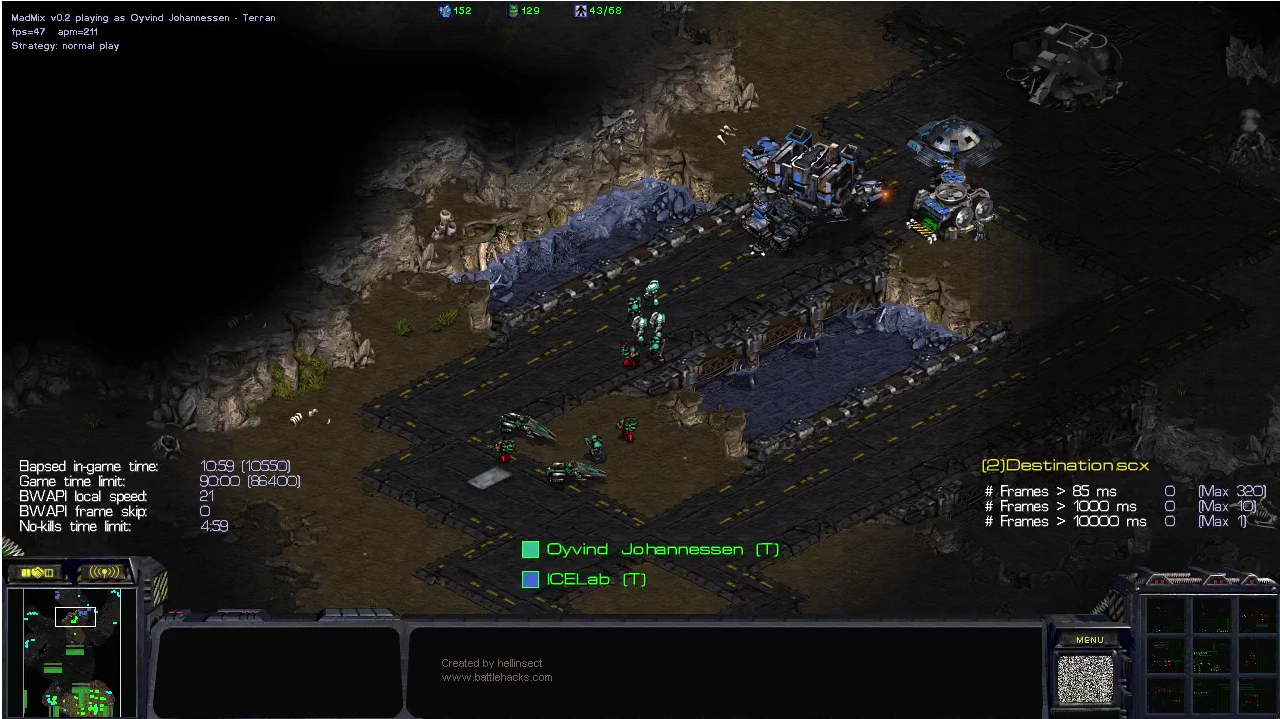
\includegraphics[width=1\columnwidth]{fig/sscait-stream.png}
  \caption{SSCAIT live stream running in HD resolution and controlled by the custom observer script~\cite{mattsson2015automatic}.}
  \label{figSSCAITstream}
\end{figure}

The activity of bot programmers and the general public surrounding SSCAIT has grown considerably over the course of the past year, with new members to the organizing team making a number of improvements to the live stream, and better community engagement during the Ladder phase.

First, the ladder phase was updated, with SSCAIT introducing so-called ``weekly reports''. Every weekend, there is a 1-2 hour long segment of curated AI vs. AI matches with insightful commentary on the live stream. Second, a voting system was implemented, allowing bot programmers and viewers to select which bots will play the next ladder match on live stream (Figure \ref{figSSCAITvoting}). This not only supports viewer engagement, but also greatly simplifies bot debugging process. Bot programmers can now quickly test their newest updates against specific opponents. This change might have contributed to the significant increase in bot update frequency. Approximately 5-6 bots are updated every day, in contrast to 0-2 updates per week in 2015.

Another update was the introduction of ``minitournaments'' to SSCAIT. These are easily configurable, irregular and unofficial short competitions, taking up to one day. The format of these minitournaments and the selection of participants is usually up to the stream viewers and moderators. Visual quality of the stream was improved by updating the custom observer script~\cite{mattsson2015automatic} which now moves the camera fluently to the most interesting parts of the game in real time and displays SSCAIT-related information on top of the game. The stream was also upgraded to HD using a ``resolution hack'' (Figure \ref{figSSCAITstream}). 
The overall number of stream views has increased to 376,920 views on Twitch.tv and additional 434,216 views on SmashCast.tv over the past 12 months. Two additional metrics were added to the ladder ranking system due to popular demand: ELO rating~\cite{elo1978rating}, which is used in adversarial games like chess, and ``SSCAIT rank'', based on so-called ``ICCUP ranking system'', typical for competitive StarCraft.

\subsubsection*{SSCAIT Tournament Phase Updates}

The 2017/18 installment of SSCAIT's tournament phase took place during four weeks at the end of December 2017 and beginning of January 2018 and sported 78 participants. The tournament was divided into two divisions:

\emph{Student Division}: Round Robin tournament of 6006 games, where every bot played two games against every opponent. Only the bots created by individual students were considered ``student'' bots and were eligible for victory in this division. Other bots were tagged as ``mixed-division'' bots (they played the games, but could not win the student division title). Winners of the student division in 2017/18 were:
  \begin{enumerate}
	\item Wulibot, University of Southern California (USA) with 124 wins
	\item LetaBot (Martin Rooijackers), University of Maastricht (Netherlands) with 109 wins
	\item Carsten Nielsen, Technical University of Denmark (Denmark) with 101 wins
  \end{enumerate}
The student division of SSCAIT exists so that the students stand a chance of winning in the presence of more experienced, non-student participants and team-created bots.

\emph{Mixed Division}: After the student division ended, sixteen bots with the most wins among all the participants were selected for the additional “mixed division” double elimination bracket, consisting of 30 matches (best of 3, 5, or 7 games), which can be seen in Figure \ref{figSSCAITbracket}. 

\begin{figure}[t] 
  \centering
  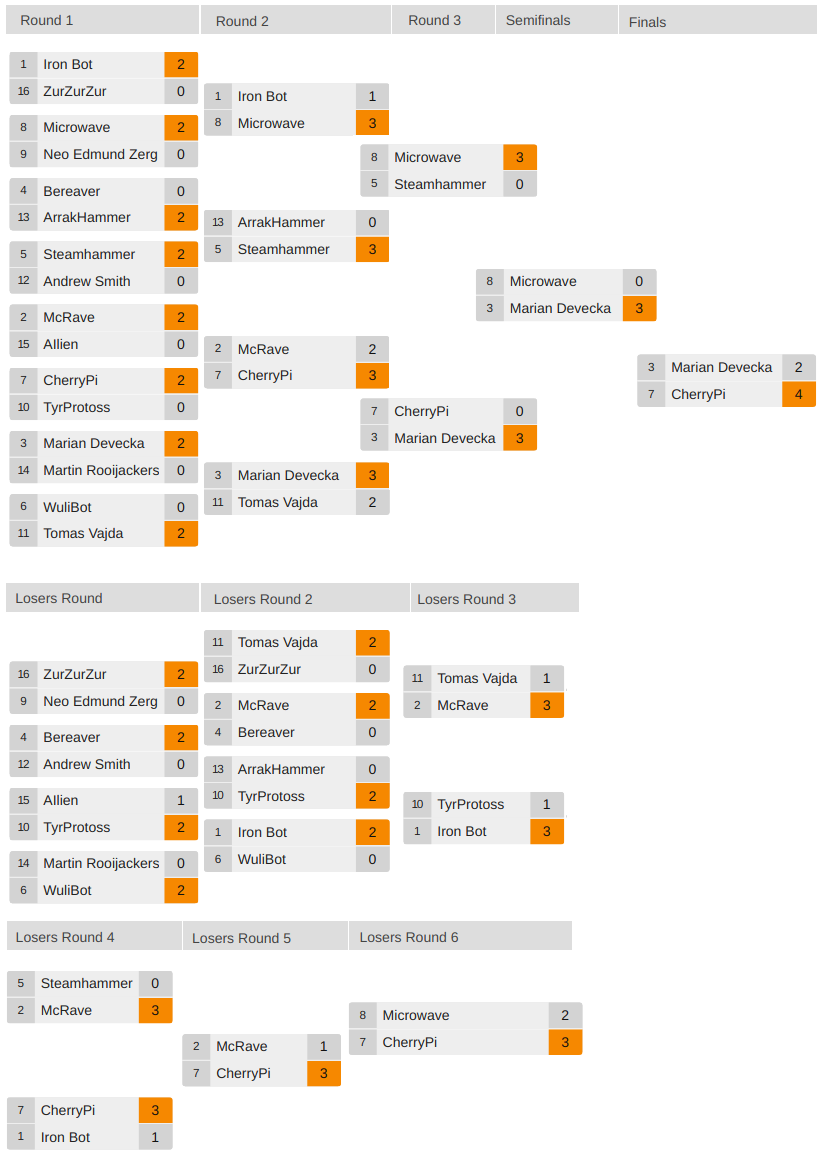
\includegraphics[width=1.04\columnwidth]{fig/sscait-bracket.png}
  \caption{SSCAIT 2017/18 mixed division double elimination bracket.}
  \label{figSSCAITbracket}
\end{figure}  

{\em CherryPi}, created by the Facebook AI Research team won the mixed division by beating KillerBot by Marian Devecka 4-2 in the finals. Interestingly, CherryPi encountered KillerBot earlier in the tournament (in winner's round 3) and lost that match 0-3, dropping down to the losers bracket. The bot then managed to win the whole losers bracket, meet Killerbot again in the finals and win by exploiting its experience from their previous games. More information about CherryPi can be found in Section~\ref{secBots}.
%{\em LetaBot} (created by Martin Rooijackers) won the mixed division elimination bracket in addition to winning the student division, after beating {\em Krasi0bot} (created by Krasimir Krystev) 3 to 1 in the finals~(fig. \ref{figSSCAITbracket}). {\em LetaBot} had hard-coded special strategies against specific opponents. It successfully executed an ``SCV rush'' in the final games -- a strategy for which {\em Krasi0bot} was not prepared. 
All the elimination bracket games were published as videos with commentary on SSCAIT YouTube channel\footnote{\url{https://goo.gl/icbYdK}} and as replay files on SSCAIT website.\footnote{\url{http://sscaitournament.com/index.php?action=2017}} 

% This is not relevant to the paper
%Tournament winner, Martin Rooijackers, has recently been invited to have a talk about this achievement at a business-oriented AI conference {\em World Summit AI}.\footnote{\url{http://worldsummit.ai/}} 




\section{AIIDE: Artificial Intelligence and Interactive Digital Entertainment}\label{subsecAIIDE}

The AIIDE Starcraft AI Competition is the longest running annual Starcraft competition, and has been held every year since 2010 along with the AAAI Artificial Intelligence and Interactive Digital Entertainment conference. Unlike the CIG and SSCAIT competitions, the AIIDE competition requires (since 2011) that bot source code be submitted, and that the code will be published for download after the competition has finished. Running 24 hours a day for 2 weeks with games played at super-human speed, the competition is a single round-robin format with the winner being the bot with the highest win percentage when the time limit has been reached. 

\subsection{AIIDE StarCraft AI Competition History}

The AIIDE Starcraft AI Competition was first run in 2010 by Ben Weber at the Expressive Intelligence Studio at University of California, Santa Cruz, as part of the AIIDE (Artificial Intelligence and Interactive Digital Entertainment) conference. A total of 26 entrants competed in four different game modes which varied from simple combat battles to the full game of Starcraft. As this was the first year of the competition, and little infrastructure had been created, each game of the tournament was run manually on two laptop computers and monitored by hand to record the results. Also, no persistent data was kept for bots to learn about opponents between matches. The 2010 competition had 4 different tournament categories in which to compete. Tournament 1 was a flat-terrain unit micro-management battle consisting of four separate unit composition games. Tournament 2 was another micro-focused game with non-trivial terrain. Tournament 3 was a tech-limited StarCraft game on a single known map with no fog-of-war enforced. Players were only allowed to choose the Protoss race, with no late game units allowed. 

Tournament 4 was considered the main event, which involved playing the complete game of StarCraft: Brood War with fog-of-war enforced. The tournament was run with a random pairing double-elimination format with each match being best of 5 games. A map pool of 5 well-known professional maps were announced to competitors in advance, with a random map being chosen for each game. Tournament 4 was won by Overmind - a Zerg bot created by a large team from the University of California, Berkeley, who defeated the Terran bot Krasi0 by Krasimir Krastev in the finals.

From 2011 to 2016, the AIIDE competition was hosted by the University of Alberta, and was organized and run each year by David Churchill and Michael Buro. Due to the low number of entries to Tournaments 1, 2, and 3 from the 2010 AIIDE competition, it was decided that the AIIDE competition for 2011 would only consist of the full game of Starcraft (with the same rules as the 2010 Tournament 4), with no smaller micromanagement tournaments. The 2011 tournament rules were also updated so that all entrants must submit the source code of their bot and allow it to be published after the competition is over, which was done for several reasons. The first reason was to lower the barrier to entry for future competitions - since programming a Starcraft AI bot was very time consuming, future entrants could download and modify the source code of previous bots to save considerable effort. Another reason was to more easily prevent cheating - with thousands of games being played in the tournament, no longer could each game be manually inspected to detect if any cheating tactics were being employed, which would be more easily detected by inspecting the source code. The final reason was to help advance the state of the art in Starcraft AI by allowing future bots to borrow strategies and techniques of previous bots by inspecting their source code - ideally, all bots in future competitions should be at least as strong as the bots from the previous year. 

Since the first competition was run by a single person on two laptops, games were played by manually starting the Starcraft game and creating and joining games by hand. As the physical demand was quite high, a simple random-pairing double-elimination tournament was played with approximately 60 games in total. This caused some negative feedback that this elimination-style tournament was quite dependent on pairing luck, so for the 2011 competition all chance was eliminated from the tournament by playing a round robin style format. Playing a round robin format requires far more games to be played, and it would no longer be possible to run each game manually. In the summer of 2011, the StarCraft AI Tournament Manager software was written (see section~\ref{secTournamentManagerSoftware}) which could automatically schedule and play round robin tournaments of Starcraft on an arbitrary number of locally networked computers. The initial version of this software allowed for a total of 2340 games to be played in the same time period as the 2010 competition's 60 games, with each bot playing each other bot a total of 30 times. There were 10 total maps in the competition, chosen from expert human tournaments that were known to be balanced for each race, which were available for download several months in advance on the competition website. The AIIDE competition was modeled on human tournaments where the map pool and opponents are known in advance in order to allow for some expert knowledge and opponent modeling. 


The 2012 AIIDE competition brought a major change to the functionality of the StarCraft AI Competitions: persistent file storage, which allowed the bots to learn throughout the course of the competition. The tournament managing software was updated so that each bot had access to a read folder and a write folder contained on a shared folder which was accessible to all the client machines. During each round bots could read from their 'read' folder and write to their 'write' folder, and at the end of each round robin (one game between each bot pairing on a single map) the contents of the write folder were copied to the read folder, giving access to all information written about previous rounds. This new functionality was used by several bots to implement strategy selection, in which their bot selected which of several strategies to use based on the results of previous rounds vs.\ the same opponent, which typically increased their win rates over time during the competitions.

%\begin{figure}[t]
%  \centering
%  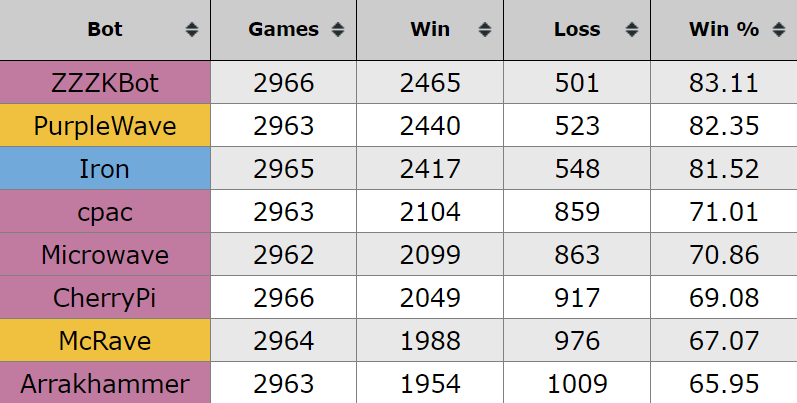
\includegraphics[width=1\columnwidth]{fig/aiide2017.png}
%  \caption{Results of the top 8 finishers in the 2017 AIIDE competition. Zerg bots are listed in purple, Terran bots in blue, and Protoss bots in yellow.}
%  \label{figAIIDEresults}
%\end{figure}

\begin{table}[t]
\begin{center}
	\begin{tabular}{| c | c | c | c | c | c |}
		\hline
		\textbf{Bot} & \textbf{Race} & \textbf{Games} & \textbf{Win} & \textbf{Loss} & \textbf{Win \%} \\
		\hline
		ZZZKBot & Zerg & 2966 & 2465 & 501 & 83.11 \\
		\hline
		PurpleWave & Protoss & 2963 & 2440 & 523 & 82.53 \\
		\hline
		Iron & Terran & 2965 & 2417 & 548 & 81.52 \\
		\hline
		cpac & Zerg & 2963 & 2104 & 859 & 71.01 \\
		\hline
		Microwave & Zerg & 2962 & 2099 & 863 & 70.86 \\
		\hline
		CherryPi & Zerg & 2966 & 2049 & 917 & 69.08 \\
		\hline
		McRave & Protoss & 2964 & 1988 & 976 & 67.07 \\
		\hline
		Arrakhammer & Zerg & 2963 & 1954 & 1009 & 65.95 \\
		\hline
 \end{tabular}
 \end{center}  
 \caption{Results of the top 8 finishers in the 2017 AIIDE competition.}
 \label{tableAIIDE}
\end{table} 

The AIIDE competitions between 2013 and 2016 did not have any major rule changes, and continued to use the same pool of 10 maps for each competition. Competition appeared to stagnate between 2011 and 2013, with a relatively low number of entrants, and saw the same 3 bots (Aiur, Skynet, and UAlbertaBot) trading 1st, 2nd, and 3rd place during these years. The 2014 to 2016 competitions however saw many new entries to the competition, with new bots taking the top 3 positions each year. Top 3 finishers of each year's competition can be seen in Table \ref{tableTournaments}. Improvements to the tournament software and hardware infrastructure allowed for more games to be played each year, which can be seen in Figure \ref{fig:comps}.

\subsection{2017 AIIDE Competition}\label{subsecAIIDEnews}

The 2017 AIIDE competition\footnote{\url{http://www.cs.mun.ca/~dchurchill/starcraftaicomp/2017/}} had a total of 28 competitors, and the round robin games ran on 14 virtual machines for two weeks. A total of 110 rounds of round robin play were completed, with each bot playing 2970 games for a total of 41580 games. Any bot that achieved a win rate of 30\% or higher in the 2016 competition which did not receive a new submission was automatically entered into the 2017 competition. No new rules or maps were used for the 2017 tournament that were not in place for the 2016 tournament. The AIIDE tournament manager software had been updated with new features, such as support for BWAPI version 4.2.0, and the ability for client machines to be listed with special properties, such as GPU computation ability. In combination with this update, a hardware upgrade for the tournament allowed for GPU computation support for any bots that required it, however no 2017 bots used the feature. The 2017 competition had the closest top 3 finish of any competition yet, with the top 3 bots separated by less than 2\% win rate, and 3rd-6th place bots also separated by less than 2\% win rate. Statistics for the top 8 finishers can be seen in table \ref{tableAIIDE}.

\begin{figure}[t]
  \centering
  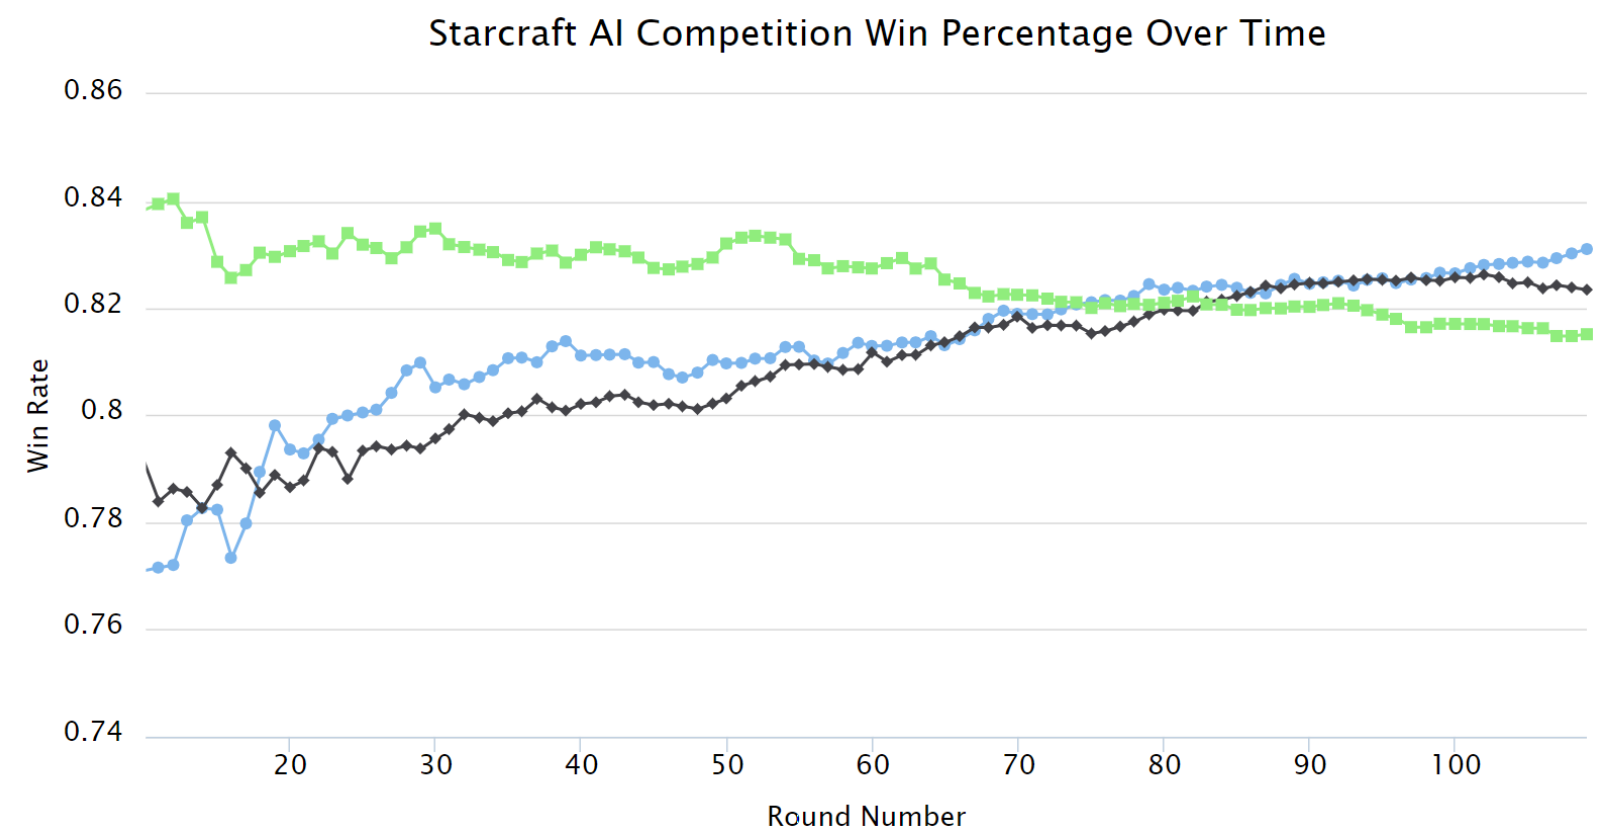
\includegraphics[width=1\columnwidth]{fig/aiideWinPerc.png}
  \caption{Win percentage over time for the top 3 bots of the 2017 AIIDE StarCraft AI Competition. 1st place ZZZKBot shown in blue, 2nd place PurpleWave in black, and 3rd place Iron in green. }
  \label{aiideWinPerc}
\end{figure}

The win percentage over time of the top 3 bots of the competition can be seen in Figure \ref{aiideWinPerc}, and demonstrates the importance of implementing some form of opening modeling / learning over time. Although Iron (shown in green) led for the vast majority of the competition, it did not implement any form of learning over the course of the competition, and its win rate slowly dropped over time. ZZZKBot (blue) and PurpleWave (black) implemented strategy selection learning, and their win rates slowly climbed to the point where they overtook Iron near round 85 of 110. 


\section{CIG: Computational\\ Intelligence in Games}\label{subsecCIG}

The CIG StarCraft AI Competition has been a part of the program of the IEEE Computational Intelligence in Games (CIG) conference since August 2011.  Since the date of the CIG competition was usually just before the AIIDE competition, many of the bots submitted to both competitions ended up being nearly identical, therefore the CIG competition has several rule differences with AIIDE in order to keep the results interesting. The biggest rule difference was that the CIG competition did not disclose which maps would be used for the competition, meaning that the bots could not use any hard-coded map information like they could for AIIDE.

\subsection{CIG Competition History}
The CIG conference is well known for hosting and organizing many AI related competitions, such as the Mario AI Competition and the General Video Game Playing Competition, and in 2010 the first CIG StarCraft AI Competition was held. Organized by Johan Hagelback, Mike Preuss, and Ben Weber, the CIG 2010 competition was to have a single game mode similar to the tech-limited Tournament 3 from the AIIDE 2010 competition, but using the Terran race instead of the Protoss race. Unfortunately the first year of the CIG competition had several technical problems, and no winner could be announced for the competition. Mike Preuss and his team members then successfully organized the CIG competition each year from 2011 to 2013. Since 2014, the Sejong University team (led by Kyung-Joong Kim) has organized the CIG  competition at the IEEE CIG conference. In order to provide a more diverse competition, CIG rules and settings have changed each year, shown in Table~\ref{tableTournaments}. 

Throughout its history, CIG has had multiple changes in the selection of tournament management software, open-source policy and map pool announcement policy. The tournament management software (see section \ref{secTournamentManagerSoftware}) is used to distribute the matches over multiple machines on the network and to automate the competition operation. Although CIG organizers developed their own JAVA-based TM sofware, the AIIDE TM has been used for the competition since 2014~(see details in Section \ref{secTournamentManagerSoftware}). Since 2016, CIG has enforced an open source code policy, and all of the bots' source code are published after the competition. Unlike the AIIDE competition, the CIG map pool was not known to the participants before the competition to promote generalization ability of the entries. However, it was found that participants usually did not exploit map knowledge, and so since 2016 maps in the CIG competition have been announced in advance. 
 
In the 2016 competition, the organizers introduced a second stage to the competition such that half of the entries advance to the second stage based on the win ratio of the first stage. This was inspired by the Simulated Car Racing Competition \cite{loiacono20102009} which adopted a two-stage competition divided into a qualification stage and a main race. Since the single-pool round robin format is based on win percentage only, it is important to get high average win ratio against all the opponents. The CIG organizers introduced two pools with the intent to reduce the chance that the top ranking bots win just by exploiting lower ranked bots to boost their win ratio. Bots were randomly split into two groups, and then the top half of bots from each group were brought together for a final stage group, to be played as round robin, with all learned information being deleted before the beginning of the final stage. 

\begin{table}[t]
\begin{center}
	\begin{tabular}{| c | c | c | c | c | c |}
		\hline
		\textbf{Bot} & \textbf{Race} & \textbf{Games} & \textbf{Win} & \textbf{Loss} & \textbf{Win \%} \\
		\hline
		ZZZKBot & Zerg & 1984 & 1628 & 356 & 82.06 \\
		\hline
		tscmoo & Random & 1992 & 1541 & 451 & 77.36 \\
		\hline
		PurpleWave & Protoss & 2021 & 1360 & 661 & 67.29 \\
		\hline
		LetaBot & Terran & 2026 & 1363 & 663 & 67.28 \\
		\hline
		UAlbertaBot & Random & 2005 & 1315 & 690 & 65.59 \\
		\hline
		Overkill & Zerg & 2024 & 1270 & 754 & 62.75 \\
		\hline
 \end{tabular}
 \end{center}  
 \caption{Results of the 2017 CIG competition final stage.}
 \label{tableCIG}
\end{table}

\subsection{2017 CIG Competition}\label{subsecCIGnews}


In the 2017 CIG competition, the two stage format was changed back to the single group format. The reason was that the participants did not seem to change their strategy to consider the two-stage tournament, and it did not seem to have much of an effect on the final results. In the future, CIG organizers consider adopting the SWISS-system widely used in the board game community. In this setting, a player does not play against all the other opponents. Instead, the participants are paired with the opponents with similar scores. Such systems usually produce final outcomes similar to round-robin while playing fewer total games. 

In 2017, CIG organizers tried to play as many games as possible, and reached 125 rounds with 190 games per round, which resulted in 23750 games in the two-round format. Currently, AI bots often use multiple pre-prepared strategies and adapt them or their selection against specific opponents. The more games played during a tournament, the more experience allows them to learn which strategies are good against which opponents. As in the 2017 AIIDE competition, many bots implemented learning strategies which dramatically increased their win rates over time. Detailed results of the top 6 bots in the competition can be seen in table \ref{tableCIG}.

After the 2017 CIG competition Sejong University organized a special event where human players were matched against the AI bots. The human players included one novice player (ladder rating around 1100), one middle-level player (around 1500), and a professional gamer: Byung-Gu Song. AI bots in the event were ZZZKBot (winner of CIG 2017), tscmoo bot (2nd place in CIG 2017) and MJBOT, an AI bot specially designed against human players. MJBOT has been developed since June 2017 by Cognition Intelligence Laboratory to beat novice/middle-level human players. Each human player played a single game against each AI bot (9 games). The novice human player lost two games against ZZZKBOT and TSCMOO, but won the game against MJBOT, which was not able to finish the game due to a programming bug. In the next session, the middle-level human player lost all three games against the AI bots. Finally, the professional human player Byung-Gu Song won against all the AI bots\footnote{\url{http://cilab.sejong.ac.kr/}}. This suggests that the AI bots have a potential to compete against novice and middle-level players, but not professionals. 

%\begin{figure}[t]
%  \centering
%  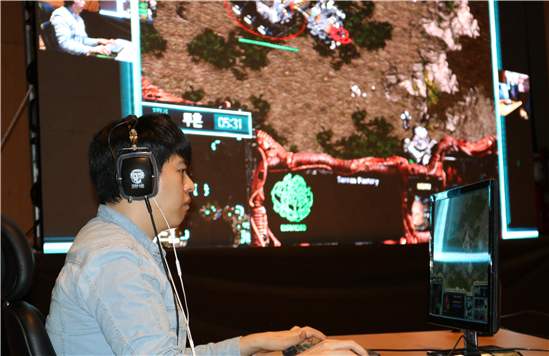
\includegraphics[width=0.5\textwidth]{fig/song_human_ai.png}
%  \caption{Professional player Byung-Gu Song playing against AI bots.}
%  \label{figureSong}
%\end{figure} 


\begin{table*}[t] 
 
 \begin{center}
 \begin{tabular} {| c | c | c c c | c c c |}
 \hline
 Competition & Year & TM Software & Open-Source & Maps & 1st Place & 2nd Place & 3rd Place\\
 \hline
 AIIDE & 2010 & Manual & Optional & Unannounced & Overmind & Krasi0 & Chronos \\
 \hline
 AIIDE & 2011 & AIIDE TM & Forced & Announced & Skynet & UAlbertaBot & Aiur \\
 \hline
 AIIDE & 2012 & AIIDE TM & Forced & Announced & Skynet & Aiur & UAlbertaBot\\
\hline
 AIIDE & 2013 & AIIDE TM & Forced & Announced & UAlbertaBot & Skynet & Aiur\\
\hline
 AIIDE & 2014 & AIIDE TM & Forced & Announced & IceBot & Ximp & LetaBot\\
\hline
 AIIDE & 2015 & AIIDE TM & Forced & Announced & tscmoo & ZZZKBot & Overkill\\
\hline
 AIIDE & 2016 & AIIDE TM & Forced & Announced & Iron & ZZZKBot & tscmoo\\
\hline
 AIIDE & 2017 & AIIDE TM & Forced & Announced & ZZZKBot & PurpleWave & Iron\\
\hline
 CIG & 2011 & Manual & Optional & Unannounced & Skynet & UAlbertaBot & Xelnaga\\
 \hline
 CIG & 2012 & AIIDE TM & Optional & Unannounced & Skynet & UAlbertaBot & Xelnaga\\
 \hline
 CIG & 2013 & Java-based TM & Optional & Unannounced & Skynet & UAlbertaBot & Aiur\\
 \hline
 CIG & 2014 & AIIDE TM & Forced & Unannounced & IceBot & Ximp & LetaBot\\
 \hline
 CIG & 2015 & AIIDE TM & Optional & Unannounced & ZZZKBot & tscmoo & Overkill\\
 \hline
 CIG & 2016 & AIIDE TM & Forced & Announced & tscmoo & Iron & LetaBot\\ 
 \hline
 CIG & 2017 & AIIDE TM & Forced & Announced & ZZZKBot & tscmoo & PurpleWave\\ 
 \hline   
 SSCAIT & 2011 & Custom & Optional & Announced & Roman Danielis & N/A & N/A\\
 \hline
 SSCAIT & 2012/13 & Custom & Optional & Announced & DementorBot & Marcin Bartnicki & UAlbertaBot\\
 \hline
 SSCAIT & 2013/14 & Custom & Optional & Announced & Ximp & WOPR & UAlbertaBot \\
 \hline
 SSCAIT & 2014/15 & AIIDE TM + Mod & Optional & Announced & LetaBot & WOPR & UAlbertaBot\\
 \hline
 SSCAIT & 2015/16 & AIIDE TM + Mod & Optional & Announced & LetaBot & Carsten Nielsen & UAlbertaBot \\
 \hline
 SSCAIT & 2016/17 & AIIDE TM + Mod & Optional & Announced & LetaBot & Wulibot & Zia Bot\\
 \hline
 SSCAIT & 2017/18 & AIIDE TM + Mod & Optional & Announced & Wulibot & LetaBot & Carsten Nielsen\\
 \hline
 \end{tabular}
 \end{center}  
 \caption{Tournament settings and top 3 finishers in the AIIDE, CIG, and SSCAIT (Student Division) competitions.}
 \label{tableTournaments}
\end{table*} 

\section{Current StarCraft Bots}\label{secBots}

Over the years, StarCraft AI competitions have motivated many individuals and groups to implement a variety of bots capable of playing complete StarCraft 1v1 games. They vary in complexity, from simple hard-coded bots, through bots employing more sophisticated AI techniques (e.g. planning), to bots capable of off-line learning (pre-training parameters in advance), or even on-line learning during the games.

In this section, we provide an overview of a selection of bots and discuss some of the AI approaches they implement. We only mention those bots that are currently active in one of the competitions, have recently been updated, and employ some more complex AI techniques. 

\begin{itemize}
  \setlength\itemsep{1em}
  
%  \item {\em AIlien:} AIlien is a relatively new Zerg bot. Various kinds of its decisions rely on ``scoring'' systems. Other than that, it employs state machines -- especially for higher-level strategy and macro decisions.
  
  \item {\em CherryPi:} CherryPi is a TorchCraft \cite{synnaeve2016torchcraft} Zerg bot developed by Facebook AI Research team. 
  It is implemented as a collection of heterogenous modules that can be added, removed, or configured via the command line. This design allows individual modules to be easily replaced with learning-powered modules, or to do narrow experiments using only a subset of them. The modules communicate by exchanging two kinds of data elements via the blackboard architecture: Key-value pairs and so-called UPC objects (Unit, Position, Command), which have a generic enough meaning to be loosely interpreted by other modules. In general, a UPC represents a probability distribution of units, a probability distribution of positions and a single command. Build orders are represented as a set of prioritized requests pushed into a queue that fills in requirements and applies optimizations (like allocating resources for just-in-time construction). Fight-or-flight decisions are made by clustering units and running a combat simulation. CherryPi's combat simulation works similarly to SparCraft simulation package (see UAlbertaBot) with a naive ``attack-the-closest-target'' policy for enemy behavior. A threat-aware path-finding is used to find the least dangerous routes to a safety. The selection of high-level strategy across multiple games is based on UCB1 algorithm, selecting from a fixed list of strategies against each race. The bot uses TorchCraft to communicate with BWAPI over TCP, which allows it to run on a different host than StarCraft.
  
  \item {\em cpac:} A Zerg bot created by a 13-person team from China, cpac combines hard-coded rules with a multi-layer perceptron network for unit production. The network is trained on state-action pairs extracted from a large data set of BroodWar games \footnote{\url{http://www.starcraftai.com/wiki/StarCraft_Brood_War_Data_Mining}}. The core of cpac bot is based on the bots UAlbertaBot and Steamhammer (see below).
  
  \item {\em ForceBot:} ForceBot is a Zerg bot written in GOAL -- an agent-based programming language designed on top of BWAPI for programming cognitive agents.\footnote{\url{http://goalapl.atlassian.net/wiki/spaces/GOAL/}} Since the GOAL language is designed to implement multi-agent systems, all of ForceBot's units have their own corresponding agent with specific beliefs and goals. Each agent more or less follows a rule-based AI pattern.  
  
%  \item {\em Ian Nicholas DaCosta:} This Protoss bot uses genetic algorithms for targeting, and detecting enemy army threat levels. Supervised learning was applied for the detection of opponent's strategies and builds.
  
  \item {\em Iron:\footnote{\url{http://bwem.sourceforge.net/Iron.html}}} Iron bot won the 2016 AIIDE competition, and is a decentralized multi-agent system, with each unit controlled by a highly autonomous individual agent, able to switch between 25 behaviors. All its units share one simple aim: go to the main enemy base and destroy it. It often seems like a harasser bot, which is due to its units having mainly individual behavior. There are also so-called ``expert'' agents who autonomously recommend how resources should be spent and what units should be trained, based on heuristics. 
  
 % \item {\em KaonBot:} For resource and unit allocation based on prioritized needs, KaonBot applies a competing priority algorithm. According to the author, the bot will learn these priorities from experience in future releases.
  
  \item {\em KillAll:} The KillAll bot is based on Overkill bot by Sijia Xu and most of its functionality is rule-based. However, its production module uses Q-learning to select unit types to produce based on the current situation. 
    
  \item {\em Krasi0bot:} Krasi0bot has competed every year since 2010, and is still being actively developed. Even though it originally started as a rule-based bot, it currently makes some use of genetic algorithms, neural networks and potential fields. Krasi0bot plays the Terran race, and is known for its strong defensive capabilities, and wide variety of strategies implemented. As Krasi0bot is not open-source, not much is known of the techniques it uses. 
  \begin{figure*}[t]
  \begin{center}
  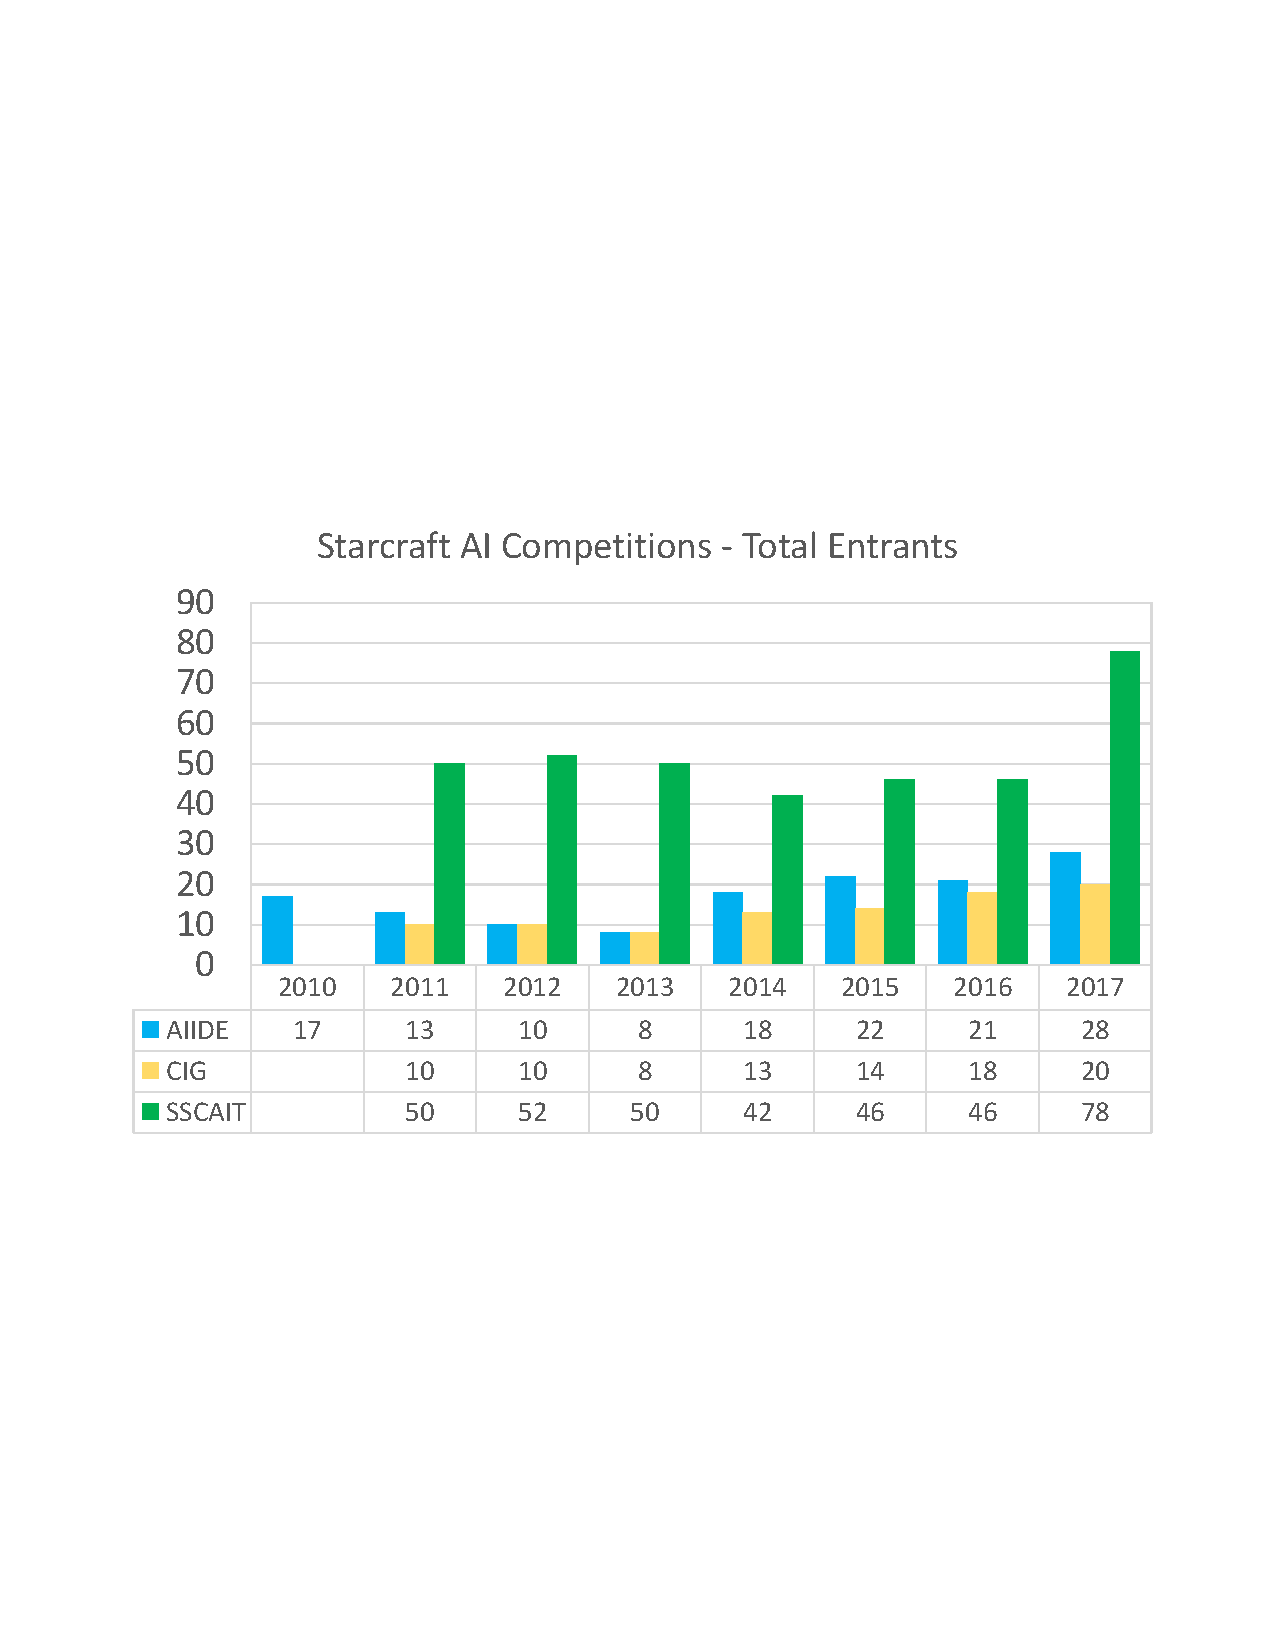
\includegraphics[width=9cm]{fig/Entrants}
	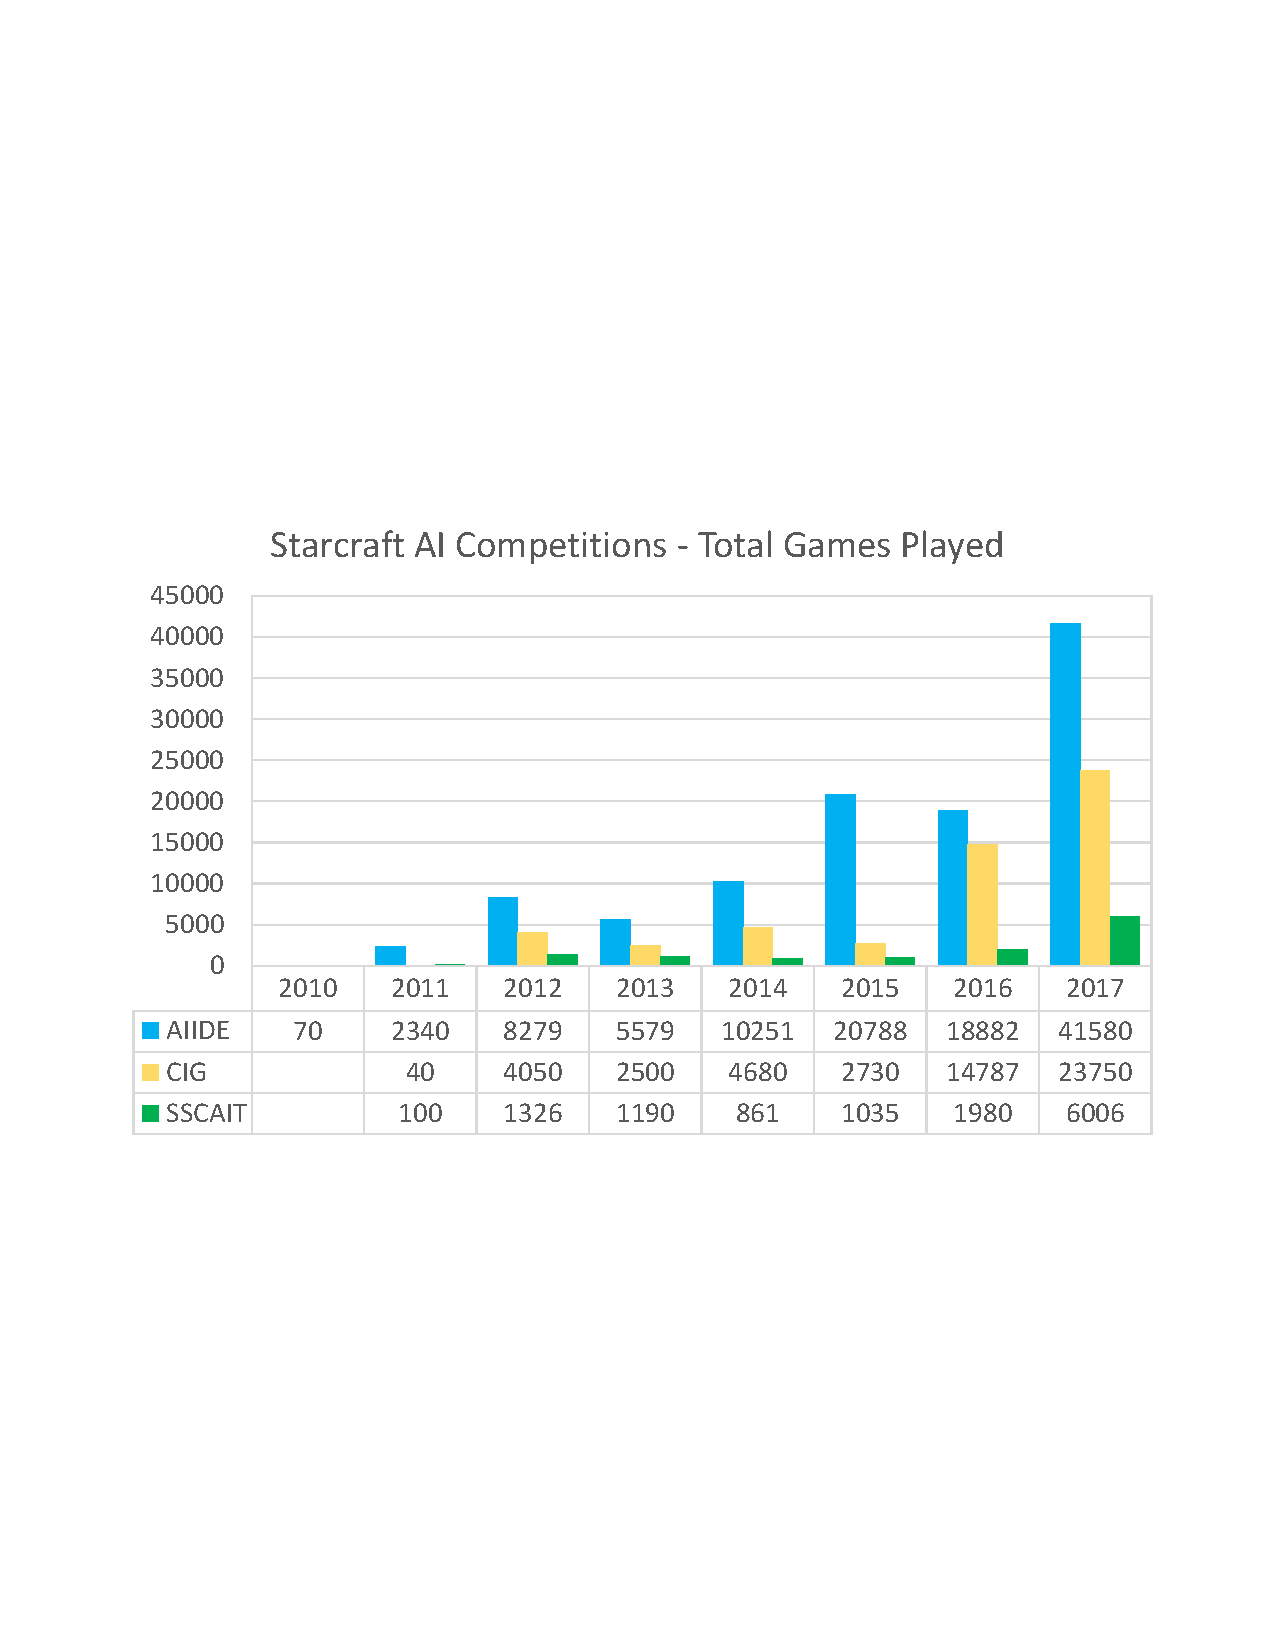
\includegraphics[width=9cm]{fig/GamesPlayed}
%  \vspace{-0.2cm}  
  \caption{Statistics for each of the 3 major annual StarCraft AI Competitions: AIIDE, CIG, and SSCAIT, since the first competition in 2010. Shown on the left is the number of total entrants for each competition, and on the right are the total number of games played in each competition.  }
  \label{fig:comps}
  \end{center}
  \vspace{-0.5cm}
\end{figure*}
  \item {\em LetaBot:\footnote{\url{https://github.com/MartinRooijackers/LetaBot}}} LetaBot won the 2014, 2015, and 2016 SSCAIT tournaments. It uses Monte Carlo Tree Search (MCTS) to plan the movement of groups of units around the map. A similar approach has previously been used by the author of Nova bot, Alberto Uriarte~\cite{uriarte2014high}. It employs cooperative pathfinding for resource gathering and text mining to extract build orders from Liquipedia articles.

  \item {\em McRave:} All the decisions of McRave bot are based on current enemy unit composition -- there are no hard-coded tech choices. The bot also builds an opponent model and uses it to select build orders. 

  \item {\em MegaBot:\footnote{\url{https://github.com/andertavares/MegaBot}}} For every game, MegaBot~\cite{tavares2016rock} chooses one of three approaches, each of which is implemented as a different bot (Skynet, Xelnaga or NUSBot). Algorithm selection is modeled as a multi-armed bandit. At the beginning of the game, an algorithm is selected using epsilon-greedy strategy. After the game, the reward is perceived (+1, 0, -1 for victory, draw and loss, respectively) and the value of the selected algorithm is updated via an incremental version of recency-weighted exponential average (Q-learning update rule).
  
%  \item {\em  Monica / Maria / Brenda:} Zerg, Protoss and Terran bots employing a game simulation inside the BEAM Erlang/OTP VM. It uses TorchCraft~\cite{synnaeve2016torchcraft}  -- a library for machine learning research on RTS games. The unit logic is written in Lua.
  
  \item {\em PurpleWave:\footnote{\url{https://github.com/dgant/PurpleWave}}} The decision making of PurpleWave bot is mainly based on hierarchical task networks. For micromanagement, it uses a hybrid squad/multi-agent approach and nearest neighbors clustering. The bot then simulates the outcomes of battles and suggests tactics for squads by min-maxing tactical approaches by each side (e.g. ``charge in'', ``run away'', or ``fight with workers''). In the end, each unit takes the tactical suggestion under advisement, but behaves independently. The units choose between approximately two dozen simple, reusable stateless behaviors. The bot heuristics include using potential fields for unit movement. Strategies are chosen based on results of previous games, race, map, and number of starting positions. It has a graph of strategy selections, like opening build orders paired with mid game transitions and late-game compositions.
  	
  \item {\em StarcraftGP:} StarcraftGP is the first StarCraft meta-bot -- a program that autonomously creates a program that autonomously plays StarCraft~\cite{garcia2015towards}. Currently, StarcraftGP v0.1 is using (Linear) Genetic Programming and it is able to directly write C++ code. Its first creations: Salsa and Tequila, have been the first bots not directly written by a human to participate in international competitions.

  \item {\em Steamhammer:\footnote{\url{http://satirist.org/ai/starcraft/steamhammer/}}} Zerg bot Steamhammer, developed by Jay Scott, and its random-race version Randomhammer both employ sophisticated combat simulation with alpha-beta search and portfolio search to predict the outcome of battles. The bots also use hierarchical reactive control for the units. For Protoss and Terran production, Randomhammer uses branch-and-bound search, while Zerg is currently rule-based.

  \item {\em tscmoo:\footnote{\url{https://github.com/tscmoo}}} tscmoo won the 2015 AIIDE and 2016 CIG competitions. The bot uses no external libraries: it has its own combat simulation code to predict the outcome of battles, it does not use BWTA\footnote{\url{http://bitbucket.org/auriarte/bwta2}} to analyze the terrain and it even has its own threat-aware path-finding for individual units. The bot is one of the most strategically diverse, and selects among its many strategies based on their success in previous games. Recent versions of the bot experimented with recurrent neural networks for high-level strategy and build order decisions.

  \item {\em UAlbertaBot:\footnote{\url{https://github.com/davechurchill/ualbertabot}}} UAlbertaBot has competed in every major StarCraft AI Competition since 2010, and won the 2013 AIIDE competition. UAlbertaBot uses a dynamic heuristic-search based Build-Order Search System (BOSS) to plan all its build-orders in real time, as well as a StarCraft combat simulation system called SparCraft for estimating the outcome of in-game battles. The bot uses the results of previous games against specific opponents to choose a strategy to implement at the beginning of each game, with each strategy being defined in an external JSON configuration file. Its development has focused on its ease of use and modification, and as such has become the basis of more than 10 other bots in current competitions, including LetaBot, Overkill, and Steamhammer. In 2017 UAlbertaBot became CommandCenter\footnote{\url{https://github.com/davechurchill/commandcenter/}}, the first bot capable of playing both BroodWar and StarCraft 2.
  
%  \item {\em V\'{a}clav Bayer:} Q-learning / Reinforcement Learning and Markov Decision Processes are used by this bot -- mainly to select a build order with respect to opponent's strategy.
  
  \item {\em ZZZKbot:\footnote{\url{https://github.com/chriscoxe/ZZZKBot}}} ZZZKBot, a Zerg bot developed by Chris Coxe, was the winner of the 2017 AIIDE and CIG competitions. Its overall strategy implements 4 simple 1-base rush strategies: 4-pool, Speedlings, Hydralisks, and Mutalisks. If the initial rush does not end the game, the bot switches to either Mutalisks or Guardians for the late game, while researching upgrades for all its units. The bot records win/loss information for each opponent, and uses this information to pick the best combination of strategy parameters for future games in a rule-based manner. The majority of the bots rules for unit control and micromanagement are simple rule-based behaviors based on expert knowledge prioritization.

\end{itemize}

%\subsection{AI Strengths and Weaknesses}

We can observe over the past few years that StarCraft AI bots are indeed getting stronger overall. In the AIIDE and CIG competitions, several bots from previous years are intentionally left in the next year to serve as a benchmark for progress, and we see each time that these benchmark bots do worse over time. Also, expert players and enthusiasts observe replays and note how they feel bots have gotten better or worse over time. Most notably, many of these expert players feel that the bots have been gradually adapting a more 'standard' playing style than earlier bots, who traditionally did one strategy such as a rush, but not much else. More modern bots have developed mid and even late game tactics that were not seen in earlier rushing bots. Overall, bots seem to be getting better at army composition, build-order selection, building placement, and overall game strategy. 

While the strongest bots currently play at an amateur human level, expert players have noted that they still appear to be weak in a few key areas. Most importantly, bots still seem quite weak at adapting their strategies dynamically during a match in response to information gained about their opponent. The majority of bots employ a playbook of several strategies that they choose from at the start of a match and follow through to the end of the game, with only a few bots attempting to dramatically change things if the opponent does something unexpected. This means that bots are still quite vulnerable to human players who are more easily able to change strategies and tactics as a game goes on. Current bots also seem quite vulnerable to the human ability to quickly identify bot patterns and behavior, and exploit this quickly during a match. For example, one human player during a human vs.\ machine match noted that one bot unit would chase his Zergling when it got close to the bots' units, and proceeded to run the Zergling next to the bot army, and then lead the bot on a wild goose chase throughout the entire map. The entire time, the bot may have been reasoning that its army could win the fight against the single Zergling unit, while not realizing that the human was just buying time until its army was ready for the final attack. This also illustrates one of the biggest challenges in all of artificial intelligence: understanding the long term effects of actions which have delayed rewards. An expert human is able to quickly understand that they are being exploited in such a way, and that it will have negative effects down the road, and is able to stop the behavior. This long-term vision that is so intuitive to humans remains a problem for current RTS AI.




\vspace{1cm}
\section{Conclusion}\label{secConclusion}

In this paper we have given an overview of the 3 major annual StarCraft AI competitions, introduced the open-source software powering them, and described some of the top performing bot participants. As seen in Figure \ref{fig:comps}, each year, participation in these competitions has continued to rise, as well as the number of games played between bots in the competitions. In the past 2-3 years, the bots in these competitions have become more strategically complex and functionally robust, employing a range of state-of-the-art AI techniques from the fields of heuristic search, machine learning, neural networks, and reinforcement learning. For many researchers, StarCraft AI competitions continue to be the environment of choice to showcase state-of-the art techniques for real-time strategic AI systems. With the increase in participation in StarCraft AI competitions, combined with the surge in activity in the field of RTS AI from hobbyist programmers, academic institutions, and industry researchers, we are hopeful that we may see a StarCraft AI capable of challenging human experts within the next few years.

 

%===================================================================================
%\section*{Acknowledgement}
%do we need to acknowledge someone?

%===================================================================================
%%% Bibliography
\bibliographystyle{IEEEtran}
\bibliography{references}{} 

\end{document}


